\documentclass[DIN,pagenumber=false,parskip=half,fromalign=left,fromphone=true,fromemail=true,fromurl=false,fromlogo=false,fromrule=false]{scrlttr2}
\usepackage[utf8]{inputenc}
\usepackage{ngerman}
\usepackage[english]{babel}
\usepackage{units}
\usepackage{tabularx}
\usepackage{booktabs}
\usepackage{multirow}
\usepackage{xcolor}
\usepackage{graphicx}
\usepackage[right]{eurosym}
\usepackage{amsmath,amsfonts,amssymb}
\usepackage{braket}
\usepackage{graphicx}
%\RequirePackage{graphicx}

\setkomavar{fromname}{Dr. Elke Faßhauer}
\setkomavar{fromaddress}{Department of Chemistry\\University of Troms\o --- The Artic University of Norway\\9037 Tromsø\\Norway}
\setkomavar{fromphone}{+47 40382485}
\setkomavar{fromemail}{elke.fasshauer@uit.no}
\setkomavar{subject}{Revision of My Article No. NJP-104327}
\setkomavar{signature}{Dr. Elke Faßhauer (corresponding author)}


\begin{document}
\begin{letter}{To the Editor}
	
	\opening{Dear Editor,}


My paper has been reviewed by two of your Referees,
who recommended it for the publication in the
New Journal of Physics subject to minor amendments.
I am thankful for the comments made by the Referees and
respond to them below. Additionally, I took the opportunity to shorten the title.

\textbf{Referee \#2} raised the following points:

\begin{enumerate}
 \item \emph{Introduction. Page 2:
             The introduction on ICD restricts the process to the prototypical
             ICD scheme of (innervalance) ionization of a cluster. I believe
             nowadays there are many more processes within the realm of ICD,
             as RICD, shakeup-ICD etc.}\\
             Also taking into account the second comment of Referee \#1:
             \emph{ICD is not only taking place after ionization. There is
             ICD after Auger, after resonant Auger, after excitation, and more.
             ICD is generally operative in nature whenever there is sufficient
             excess electronic energy in a system to ionize a neighboring atom
             or molecule. I assume that the author wanted to be brief. I
             suggest that a general statement as above is given first and then
             the author mentions that the work here concentrates on
             ionization.}\\
             the first two paragraphs of the Introduction was changed to:\\
{\color{blue}{The Interatomic Coulombic Decay (ICD) is an electronic decay process of an atom or
molecule with a sub-outer-valence vacancy involving atoms or
molecules of the environment. The decay process is initiated by the creation
of the vacancy, which can be achieved in different ways, out of which
direct ionization, excitation, an Auger decay and radioactive decay are the
most common ones. They are connected to different members of the family
of ICD-like processes such as the Electron Transfer Mediated Decay (ETMD),
the Resonance ICD (RICD), the ICD of multiply charged species like after
an Auger decay and the classical ICD (see Ref. [1, 2]
and references therein).
In this paper the classical ICD of
a sub-outer-valence
vacancy in an atom or a molecule (a unit $A$) will be discussed. After the
creation of the vacancy in $A$, it}} is filled
by an electron of the same unit and the excess energy (often called the energy of
a virtual photon $\omega_{vp}$) is transferred to a decay
partner $B$, which subsequently gets ionized:

\begin{equation*}
 A^{*+} + B \rightarrow A^+ + B^+ + e^-_{ICD}  .
\end{equation*}

In the final state,
the two units $A$ and $B$ are both positively charged, repell each other and
thereby undergo a Coulomb explosion. This process was predicted theoretically
[3], {\color{blue}{later
the first experimental evidence was found in
[4, 5] and the experimental prove was given by Jahnke et al.
[6]. Since then
it has been studied in a multitude of different systems such as small and large
rare gas clusters [7, 8, 9, 10, 11, 12, 13, 14, 15],}}
clusters of small molecules [16, 17, 18, 19, 20],
quantum dots [21], proteins [22], it is expected
to play a role in DNA damage in radiation therapy [23]
and may be used to destroy malign tissue [24, 25].

 \item \emph{It is stated, that the existence of ICD was proven in [2]. The reference is typically such, that first evidence was found in [2], the prove was given by Jahnke et al. Phys. Rev. Lett. 93, 163401. Reference [6] is typically cited, as well, as one of the experiments that showed the occurence of ICD for the first time.}\\
I changed the citation, see point 1.

 \item \emph{``The energy criterion requires energy conservation to hold'' is a somewhat strange way to describe the fact that ``a decay can only happen if the energy suffices''}\\
       The sentence was changed to:\\
       The energy criterion {\color{blue}{is a rephrasing of the energy
       conservation stating that a decay can only
       happen if the energy suffices.}}

\item \emph{Maybe ``the decay widths ... were considered to be negligible'' should be changed into something like ``decays with partner further away were considered negligible due to their decay width''.}\\
       The sentence was changed accordingly. 

\item \emph{Who is we in a single author paper? (I am aware, that I sounds very strange in a scientific publication, but maybe the according sentences can be amended in order to avoid we or I.}\\
      The formulations were kept using ``we'', because a rephrasing to passive
      voice would have made the sentence overcomplicated and compromized
      comprehensibility.

\item \emph{``..the gaseous state of their components allows for a convenient cleaning... higher count rates and therefore higher resolution..'': I do not understand this sentence and I am not sure it is actually right. Maybe an experimental collaborator can help here. (Maybe it is already enough to state, that in an experiment it helps, as well, to have a homogenous, and easily controlable target.)}
      The sentence was changed to:\\
      Their spherical
symmetry and their very localized orbitals allow for an comparably easy
theoretical description of the decay processes.
{\color{blue}{The experimental techniques to produce rare gas clusters
are well established
via variety of experimental and theoretical studies
[29, 30, 31, 5]. This makes these clusters a convenient target with controlled and predictable cluster conditions available at sufficient target densities for extended time periods as required in the here described experiments.}}

\item \emph{The Van der Waals radii do not have units.}\\
      The units were added.

\item \emph{I suggest to add horizontal lines for the different internuclear distances, as that way the statement of a decreasing energy difference for larger distances becomes clear at first glance.}\\
      The horizontal lines were added to the figure.

\item \emph{I am afraid I do not understand the last two sentences of the paragraph prior to section 5. Maybe the author can rephrase them?}\\
      The sentences were changed to:\\
      This means that for small interatomic distances and
comparably low kinetic energies of the ICD electron, the
{\color{blue}{energy}} spectrum
has a higher resolution {\color{blue}{of the interatomic distances}}.
Therefore, a peak structure might be visible for the decay with nearest
neighbours (or the closest atoms with energetically allowed decay channels)
but not necessarily for all different kinds of interaction partners at larger
distances.
\end{enumerate}

\textbf{Referee \#1} raised the following points:

\begin{enumerate}
 \item \emph{Abstract. Agreement and disagreement with experiment is addressed. Which experiment? That in [6] or that in [12]? The clusters in [12] do not correspond to those addressed here. The clusters in [6] are very large compared to the one studied here and I wonder about the comparison and the conclusion drawn (see also below).}\\
       The experiment in the former Ref. [6]. The citation was explicitly added to the
       abstract. The paper now also contains the discussion the lifetimes
       in larger clusters (see below) and the statement of the abstract is still valid.
       Therefore no further changes were applied.

 \item See comment 1 of Referee \#2.
 \item \emph{The author writes: “It was shown in earlier studies [25, 12, 26] that decay pathways with decay partners at larger distances need to be included...”. I suggest that the works by Kryzhevoi on ICD in He droplets are mentioned here too.}\\
       The additional reference was added.

 \item \emph{Page 5. The 1/R6 behavior of the decay rates is mentioned and employed. The author should mention that at distances shorter than asymptotic the rates can be substantially larger (see, e.g., the case of Ne..Mg). In rare gases the 1/R6 behavior is probably adequate (are there calculations of $\Gamma$ as a function of R for a rare gas dimer like Ne..Ne ?).}\\
       The \emph{asymptotic} $1/R^6$-behaviour is mentioned to discuss the
       behaviour at large distances. However, as mentioned in the computational
       details, this approximation is not employed in this work. Instead, a
       fit to the respective computed decay width is used. Therefore, no
       changes were applied.

 \item \emph{Page 9. The author writes: “Therefore, we consider the influence of nuclear dynamics on the lifetime to be sufficiently small to be able to neglect them in clusters in a first description. [5, 6] However, in
clusters the nuclear motion might not be fast enough to play...”. The “However” is unclear. Both sentences actually say the same.}\\
       The second sentence starting with \emph{However, } was removed.

 \item \emph{Page 5. The author takes recourse to “set 3” and “set 5”. What are these sets? It cannot be expected that the reader should search in ref. [12] to find out what is meant here. Some explanatory text is needed.}\\
       The explanatory text is already part of the manuscript and to be found
       in the sentence the Referee is referring to and the following sentence.
       Therefore, no changes were applied.

 \item \emph{Figs. 4 and 5. The author should explain in simple words how these spectra were obtained. E.g., was it assumed that each atom in the cluster is initially inner-valence ionized with the same probability?}\\
       The results were obtained with the pairwise approximation, which treats
       all pairs with the same distance in the same way. This holds for every
       calculation and therefore, to make this more clear, the computational
       details were changed accordingly and now read:\\
The calculations to obtain the ICD electron spectra of all cluster
structures were performed with
the program HARDRoC [42]
{\color{blue}{based on the decomposition of the cluster into
pairs. Every pair with the same distance is treated equally. This includes the
assumption that every neon atom is ionized with the same probability.}}
It uses experimental ionization energies shown
in Table 1 and curves fitted to the decay width of the
NeNe ICD of Ref. [10] and the NeAr decay widths of Ref.
[15]. These fitted curves yield lifetimes
$\tau=\frac{\hbar}{\Gamma}$ at the corresponding equilibrium distances of         
$\tau_{NeNe}= \unit[60]{fs}$ and                                    
$\tau_{NeAr}= \unit[44]{fs}$.

 \item \emph{Fig. 4. In the experiments ([12]) the peak at around 3 eV is well seen, while here it is there but not too intense. Can this be explained?}\\
       Yes, it can be explained. Around 3 eV many minor peaks are to be found which
       are very close in energy. Folding the spectrum adds all these contributions
       up and they appear as a peak or shoulder. The caption of Fig. 4 was
       therefore appended by:\\
          In this representation the contribution of the
          peaks around \unit[3]{eV} is easily underestimated. After folding the
          spectrum with many close lying small peaks they will add up to yield
          a visible peak or shoulder (compare Ref. [15]).

 \item \emph{Will a similar explanation make the visibility of the respective peak in Fig. 5 visible in experiment?}\\
       It is visible in the experiment, which is discussed in the text. To illustrate
       it I add a figure from \emph{Chem. Phys.} \textbf{329}, 246 (2006) with
       the non-nearest neighbour ICD highlighted in blue:
       \begin{center}
        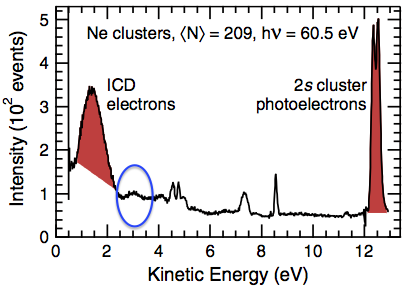
\includegraphics[]{../pics/exp_Ne_coinc_spec.png}
       \end{center}
       The larger the clusters are, the more pronounced the shoulder will be.
       In order to make the shoulder in Fig. 5 better visible, the spectra have
       been folded and incorporated in Fig. 5.

 \item \emph{I suggest to add a nice picture of the two ideal Ne clusters studied.}\\
       The pictures were added.

 \item \emph{Is the geometry of the ideal clusters optimized? Will an optimization change the picture?}\\
       The geometries of the idealized clusters presented are not optimized.
       After optimization of the structures with a force field, the distance pattern
       changed while the overall structure remained. In case of the cuboctahedral cluster
       the nearest neighbours were no longer described by only one distance but by
       different distances that are very close to the original one. In case of the
       icosahedral structure the distance pattern was split into a few characteristic
       distances, which are wider spread than in case of the cuboctahedral cluster.
       Therefore that statement that the underlying cluster structure might be
       determined by the number of peaks or without a high resolution by the width
       of the peak (the width of the icosahedral structure is larger) is unaffected.

 \item \emph{Page 12. “Two experimental ICD electron spectra of clusters with a mean cluster size < N > between 47 and 512 atoms are available...”. What does the word “between” mean here?}\\
       The spectra have been measured for mean cluster sizes between these two
       numbers. However, they were only displayed in the literature for $<N>=70$
       and $<N>=209$. Therefore, the sentence was changed to:\\
       Two experimental ICD electron spectra of clusters
       with a mean cluster size $<N>$ {\color{blue}{of 70 and 209}} atoms
       are available in the literature.
       [4, 48]

 \item \emph{Page 11. “The experimentally determined lifetimes are ...”. It is misleading to compare these experimental values with those computed for the 55 atom clusters without further discussion, like directly mentioning the size of the cluster in experiment. The whole discussion on pages 11/12 will benefit from a somewhat more coherent rewriting. I also think that if the clusters used in experiment are large and a bit unstructured (I mean that the cluster is not in its ground state structure; what was the temperature?), then there might be many atoms on the surface which may have fewer neighbors than in an idealized structure. This may also lead to longer ICD lifetimes for some of the surface atoms. May even be that the distance between atoms on the surface is different (larger) than in the bulk (?). I agree that the issue is not simple.}\\
       The experimentally investigated clusters have a mean cluster size of 900
       atoms. Therefore, I simulated the decay widths /lifetimes for clusters
       consisting of 923 atoms and added the results to the discussion.
       As expected and discussed in first manuscript, the lifetimes of the bulk
       atoms are hardly affected by the cluster size while the lifetimes of the
       surface atoms is shorter for the larger clusters. The temperature might
       indeed lead to different cluster structures. It's quantification will be
       left as a subject to future work.
       The lifetime discussion now reads:\\
{\color{blue}{We study two cluster structures,
where one has an
idealized icosahedral and the other one has an idealized cuboctahedral structure
for clusters of both \unit[55]{atoms} and \unit[923]{atoms}.
They hence consist of 13 (561) core and 42 (362) surface atoms. It was predicted
theoretically and proven experimentally that the lifetimes of ionized bulk atoms
is shorter than of ionized surface atoms due to the smaller number of direct
neighbours of surface atoms. [9, 5]
The experimentally determined lifetimes are
$\tau_{surf} = \unit[30]{fs}$ and $\tau_{bulk} = \unit[6\pm 1]{fs}$.
For our \unit[55]{atom} and \unit[923]{atom} cluster the decay widths and lifetimes
are listed in Table 2.

%\begin{table}[h]
% \centering
% \caption{Calculated decay widths and lifetimes of bulk and surface atoms
%          for icosahedral and cuboctahedral clusters of 55 and 923 atoms.}
% \begin{tabular}{llrrr}
%  \toprule
%               &                            & atoms & $\Gamma$ [meV] & $\tau$ [fs]\\
%  \midrule
%   \multirow{4}{*}{icosahedral}   & bulk    &   55  &   125          & 5.3 \\
%                                  & surface &   55  &    67          & 9.8 \\
%                                  & bulk    &  923  &   126          & 5.2 \\
%                                  & surface &  923  &    81          & 8.1 \\
%  \midrule
%   \multirow{4}{*}{cuboctahedral} & bulk    &   55  &   140          & 4.7 \\
%                                  & surface &   55  &    78          & 8.4 \\
%                                  & bulk    &  923  &   147          & 4.5 \\
%                                  & surface &  923  &    95          & 7.0 \\
%  \bottomrule
% \end{tabular}
% \label{table:lifetimes}
%\end{table}

In all cases, our results confirm the shorter lifetimes of the bulk atoms compared
to the surface atoms. Both for the icosahedral and for the cuboctahedral cluster
structure the lifetime of the bulk atoms is almost independent of the cluster size
and the difference is maximum \unit[0.2]{fs}. This can be explained by the very
similar environments of bulk atoms in smaller and larger clusters.}}
The lifetimes of the surface atoms however are smaller for the larger cluster sizes.
In small clusters, the number of face surface atoms is small compared to the
number of edge and vertex atoms in the surface. The larger the clusters are,
the larger is the relative number of the surface atoms. These surface atoms
in face positions have more direct neighbours than atoms in vertex positions.
Therefore, our estimated lifetime of the average surface atoms in the small       
clusters should be slightly larger than in larger clusters.

For both the icosahedral and the cuboctahedral cluster structures the lifetimes
of the bulk atoms are in excellent agreement with experiment.
However, the theoretical lifetimes of the surface atoms are significantly
smaller than the experimental lifetime. Assuming that the
experimental lifetimes are correct, we have to consider three error sources:      
1. the nuclear motion excluded in our approach, 2. different cluster structures,  
and 3. a different stabilization of charges between the             
inner-valence ionized and the outer-valence ionized atom compared to the bulk.    
                                                                    
{\color{blue}{
Cluster structures with larger interatomic distances of the surface atoms between 
each other and the core atoms would explain the higher experimental lifetimes of  
the surface atoms. These could be caused by non-ideal structures due to the       
clusters' temperature.}} ...

 \item \emph{I wonder what happens in a relatively big idealized cluster if one computes the influence of all neighbors (like done in the He droplets)? If the distances are optimized? After all, there will then be very many contributors and as the Coulomb repulsion falls off ‘rapidly’ with distance, the energy of the ICD electron will not spread too much. The number of neighbors on a sphere of Radius R from a given atom grows as R2 and the rate falls as 1/R6 implying that the total fall off is only as 1/R4. Can this explain the question in point 8 above?}\\
      Throughout the entire work, the decay widths were simulated using the decay
      with all possible decay partners.
      ICD electron spectra of large neon clusters (8217 atoms) were
      calculated and the spectrum does
      hardly change qualitatively compared to the spectra of 55 atoms. ICD electrons
      at higher energies up to \unit[5.37]{eV} are observed with a low probability and the
      contribution of the decay with nonnearest neighbours is slightly increased.
      
      To explain the decrease of the decay by an $R^{-4}$-behaviour is an interesting
      ansatz. However, it oversimplifies the problem.
      The surface of the sphere is proportional to $R^2$, but on this surface several
      3D objects have to be placed, which in addition have the projection of a circle.
      Therefore, it is impossible to cover the entire surface of the sphere and
      the number of atoms per shell is smaller than a $R^2$-behaviour would suggest.
      It is though
      proportional to the square of the number of atoms per edge $c$
      (which can be used as an alternative measure of $R$) of the respective
      outermost shell. The number of the outermost
      shell ($os$) of a cluster with edge length $c$ can be established from 
      the total number of atoms per cluster

      \begin{equation*}
       n_{atoms,total} = \frac{10}{3} c^3 - 5 c^2 + \frac{11}{3} c -1 .
      \end{equation*}

      The number of atoms in the outermost shell is then given by
      \begin{align*}
       n_{os} &= n(c) - n(c-1)\\
              &= 10 c^2 - 20c + 12 .
      \end{align*}

      Additionally, both the icosahedral and the cuboctahedral clusters are not
      perfect spheres. This also means that, except for the first shell,
      atoms in the same shell, depending on the
      character of their position, have different distances to the central atom and
      hence correspond to different peaks in the spectrum.

      In order to illustrate this,
      please find a calculated spectrum of an excited central neon atom in cuboctahedral
      neon cluster with 14 atoms per edge (8217 atoms in total) plotted in a logarithmic
      scale:
       
      \begin{center}
       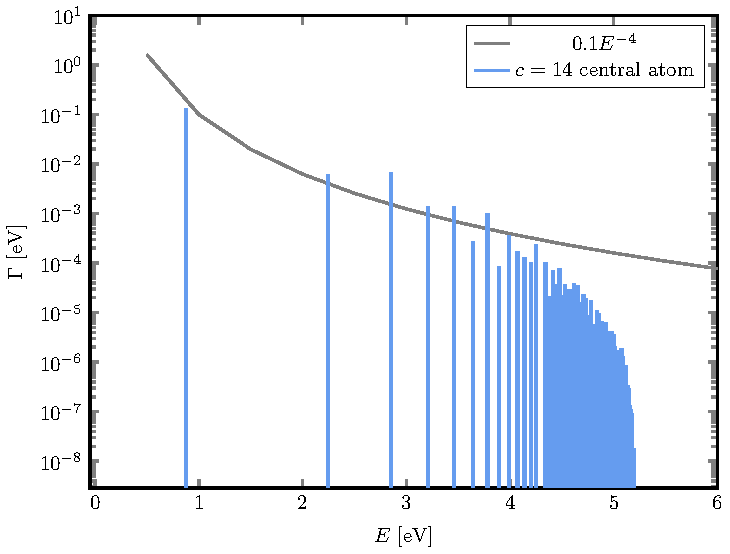
\includegraphics[width=0.7\textwidth]{../pics/center.pdf}
      \end{center}
      The first peak corresponds to decay partners in the first shell, but the
      next three peaks correspond to the second shell, the next five to the third
      shell etc. The further the shell is away, the more it is split into
      different distances. This makes a fit to the above equation unreasonable.

      Another feature of clusters is visible in this spectrum: the non-infinite
      dimension of clusters. The spectrum ends at \unit[5.19]{eV}, which would not occur
      in a solid state environment. However, these decays with partners at distances
      above \unit[80]{\AA} would be highly unlikely.

      This discussion holds for the optimized structures as well.

\end{enumerate}


I took the opportunity to shorten the title in order to not highlight only
one out of several aspects. It now reads:\\
      Non-nearest Neighbour ICD in 
      Clusters


        \closing{Sincerely yours,}
	\end{letter}

\end{document}
